\documentclass{beamer}
\usetheme{metropolis}
\usepackage{graphicx}
\usepackage{amsmath}
\usepackage{hyperref}
\usepackage{tikz}
\usetikzlibrary{circuits.ee.IEC,positioning}
\usepackage{pgfplots}
\pgfplotsset{compat=1.18}
\title{Reliability Engineering 101 for NSWC Corona}
\author{Jordan Hanson}
\institute{Whittier College Department of Physics and Astronomy}
\definecolor{mBlack}{RGB}{0,0,0}
\definecolor{mGray}{RGB}{64,64,64}
\setbeamercolor{normal text}{fg=mBlack}
\setbeamercolor{alerted text}{fg=mGray}

\begin{document}
\maketitle

\begin{frame}{Outline}
\small
\textbf{Part I : Introduction and Mathematics}
\begin{itemize}
\item 1.1 : Scope of Reliability Engineering
\begin{itemize}
\item 1.1.1 : NAVSEA Documentation on Reliability
\item 1.1.2 : Impact of Reliability
\item 1.1.3 : Knowing our Systems
\item 1.1.4 : Model and Method Selection
\item 1.1.5 : Model Development
\end{itemize}
\item 1.2 : Mathematics of Reliability Engineering
\begin{itemize}
\item 1.2.1 : Statistics and Probability
\item 1.2.2 : Probability Distribution Functions (PDFs)
\item 1.2.3 : Estimation and Hypotheses Testing
\item 1.2.4 : Graphical and Tabular Methods
\item 1.2.5 : Goodness-of-Fit Tests
\item 1.2.6 : Regression Analysis
\end{itemize}
\end{itemize}\end{frame}
\begin{frame}{Outline}
\small
\textbf{Part II : Reliability of Components and Systems}
\begin{itemize}
\item 2.1 : Reliability of Components
\begin{itemize}
\item 2.1.1 : Reliability Functions : $f(t)$, $F(t)$, $R(t)$, and $h(t)$
\item 2.1.2 : Common PDFs for Reliability Functions
\item 2.1.3 : Model Selection and Parameter Estimation
\begin{itemize}
\item Application of Maximum-Likelihood Estimators (MLEs)
\item Non-parametric Estimators
\item Bayesian Techniques
\end{itemize}
\end{itemize}
\item 2.2 : Reliability of Systems
\begin{itemize}
\item 2.2.1 : Reliability Block Diagrams (RBDs)
\item 2.2.2 : Success and Fault Tree Analysis
\item 2.2.3 : Failure Mode and Effect Analysis (FMEA/FMECA)
\end{itemize}
\end{itemize}
\end{frame}
\begin{frame}{Outline}
\small
\textbf{Part III : Reliability and Availability of Repairable Systems}
\begin{itemize}
\item 3.1 : Reliability of Repairable Systems
\begin{itemize}
\item 3.1.1 : Point Process Definition and Homogeneous Point Processes (HPPs)
\item 3.1.2 : Non-Homogeneous Point Processes (NHPPs) and Renewal Processes
\item 3.1.3 : Analysis Techniques for HPPs and NHPPs
\item 3.1.4 : Availability of Repairable Systems
\item 3.1.5 : Availability of Complex Systems
\end{itemize}
\item 3.2 : Selected Topics in Reliability Data Analysis
\begin{itemize}
\item 3.2.1 : System Classification (One-shot, repairable)
\item 3.2.2 : Reliability Data, Type and Classification
\end{itemize}
\end{itemize}
\end{frame}

\section{Part I: Introduction and Mathematics}

\section{Module 1.1 : Scope of Reliability Engineering}

\begin{frame}{Module 1.1.1 :  NAVSEA Documentation on Reliability}
\textbf{Reliability Engineering : } \textit{When you engage the ignition in your vehicle in the morning, how do you know it will work?} \\ \vspace{0.5cm}
\small
\textbf{Example documentation : }
\begin{itemize}
\item ``A Simplified Technical Guide for System Reliability: A Reliability Planning and Deployment Reference for Acquisition Professionals.'' (Section 219 Project, 2019, Port Hueneme/NAWC China Lake/NSWC Corona)
\item \textit{System Reliability Toolkit-V}. \textit{Quanterion Solutions Inc., 2015.}
\item O'Conner and Kleyner : \textit{Practical Reliability Engineering.} Wiley and Sons (2012).
\item Modarres, Kaminskiy, and Krivstov : \textit{Reliability Engineering and Risk Analysis, 3rd Ed.} CRC Press (2017). 
\end{itemize}
\end{frame}

\begin{frame}{Module 1.1.2 : Impact of Reliability}
\small
\begin{itemize}
\item \textbf{Reliability drives efficient programmatic decisions.}
\begin{itemize}
\scriptsize
\item Evidence-based acquisition activities
\item Optimization of design features and cost versus risk
\item Identification of design flaws and manufacturing defects
\item Enhancement of reliable system service-life
\end{itemize}
\end{itemize}
\begin{figure}
\centering
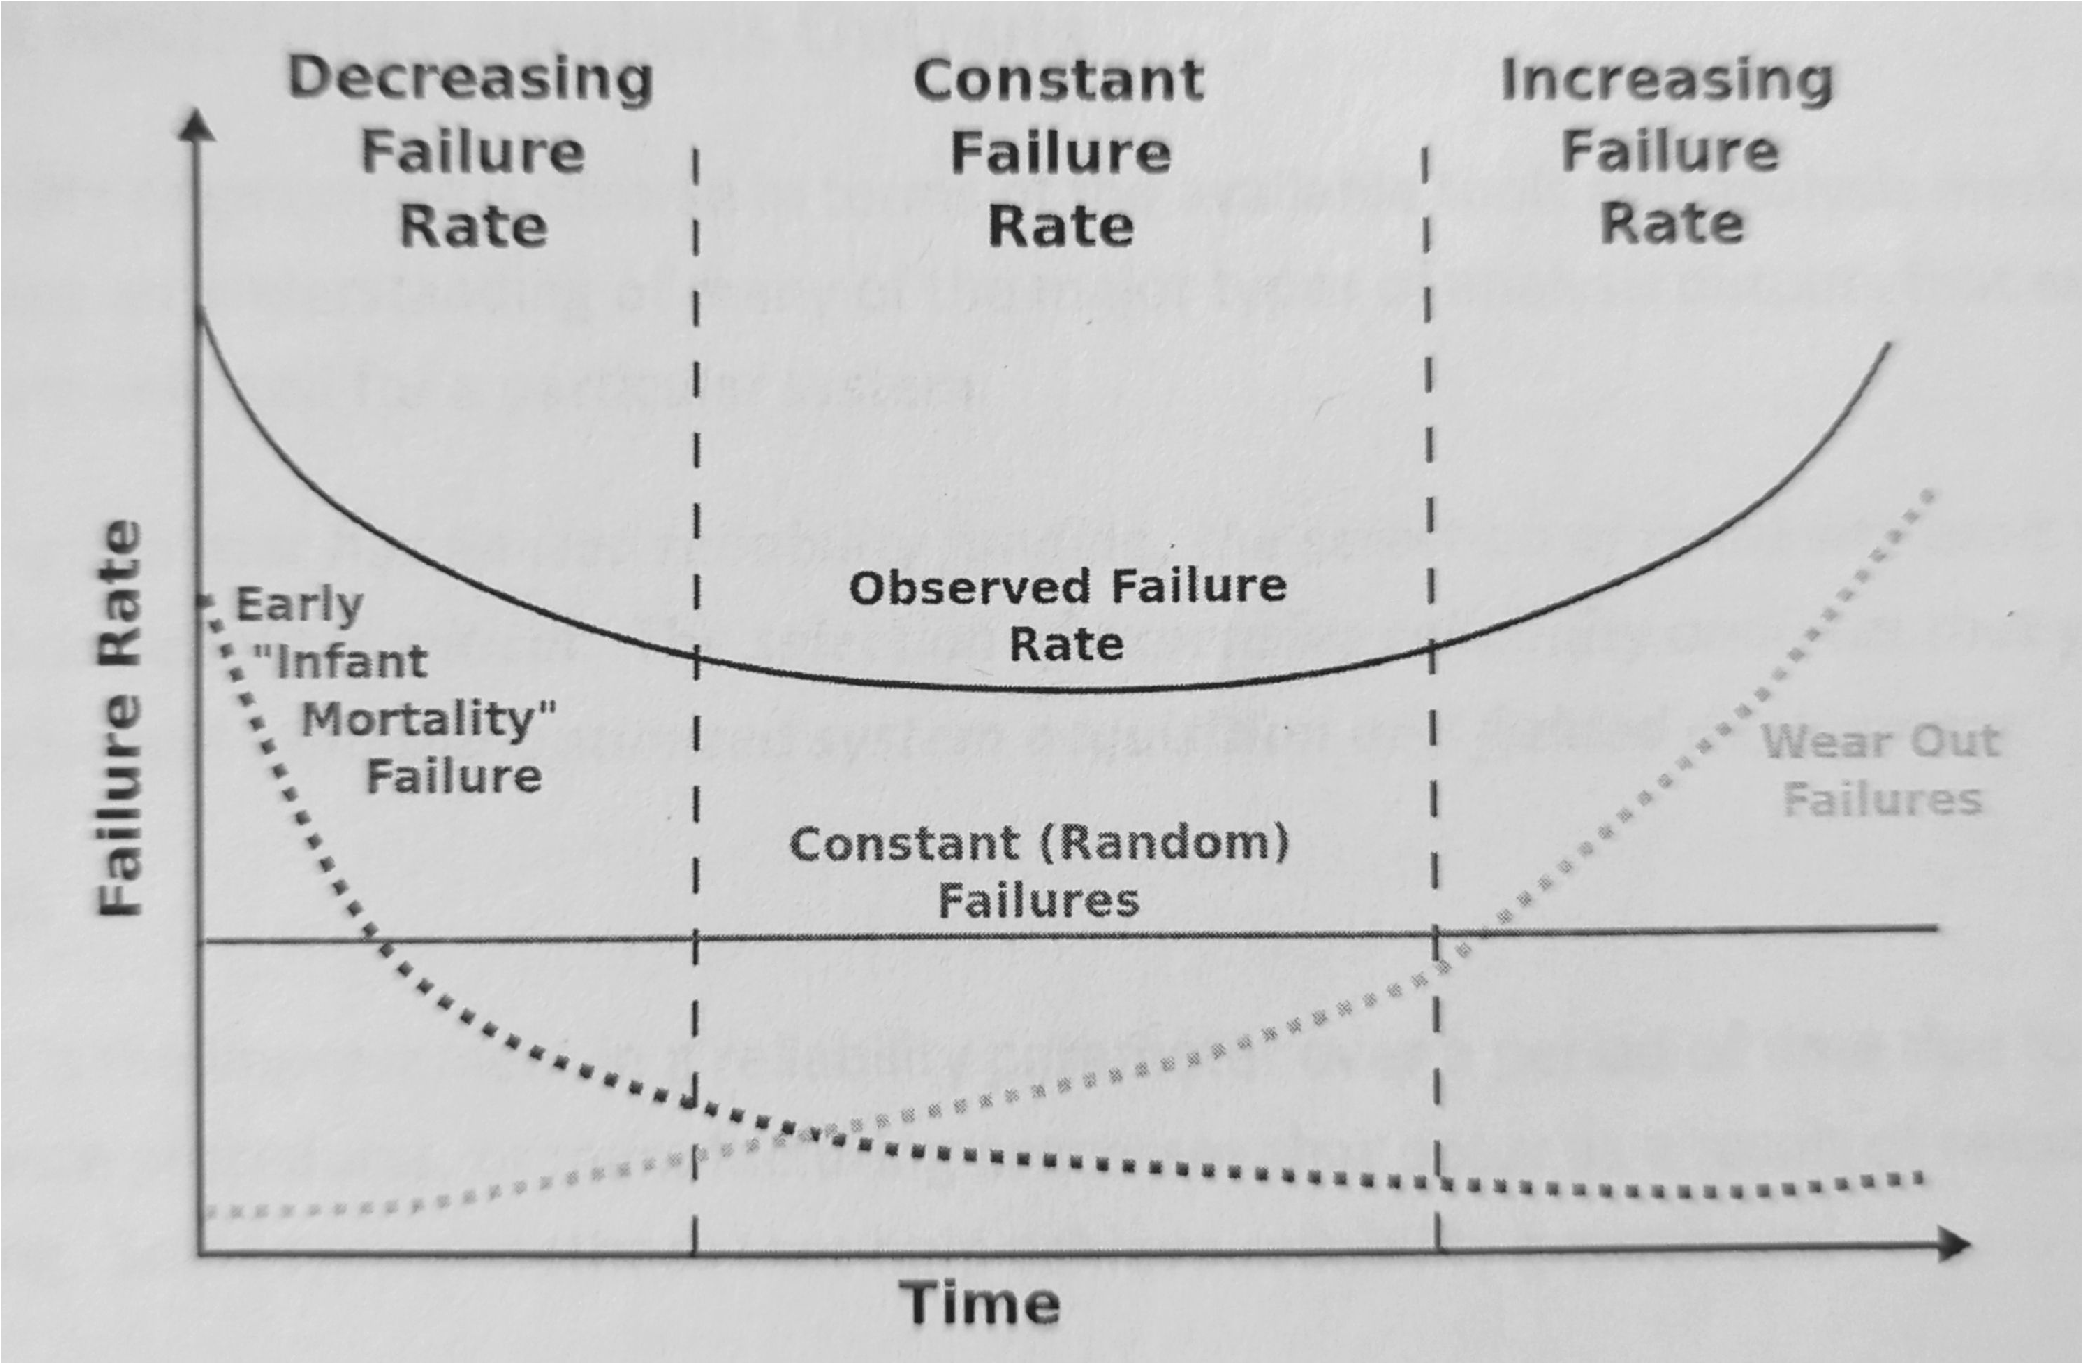
\includegraphics[width=0.75\linewidth]{bathtubCurve.pdf}
\end{figure}
\end{frame}

\begin{frame}{Module 1.1.2 : Impact of Reliability}
\small
\textbf{Reliability engineering addresses different system types.}
\begin{itemize}
\scriptsize
\item \textit{Impulse untestable systems} : must be irreversibly expended to measure their current state (operational or failed) to assess reliability.
\item \textit{Impulse testable systems} : the system must be tested to know its state (operational or failed), and testing can take place at sparse intervals
\item \textit{Continuous use systems} : the system state (operational or failed) is always known
\end{itemize}
\begin{figure}
\centering
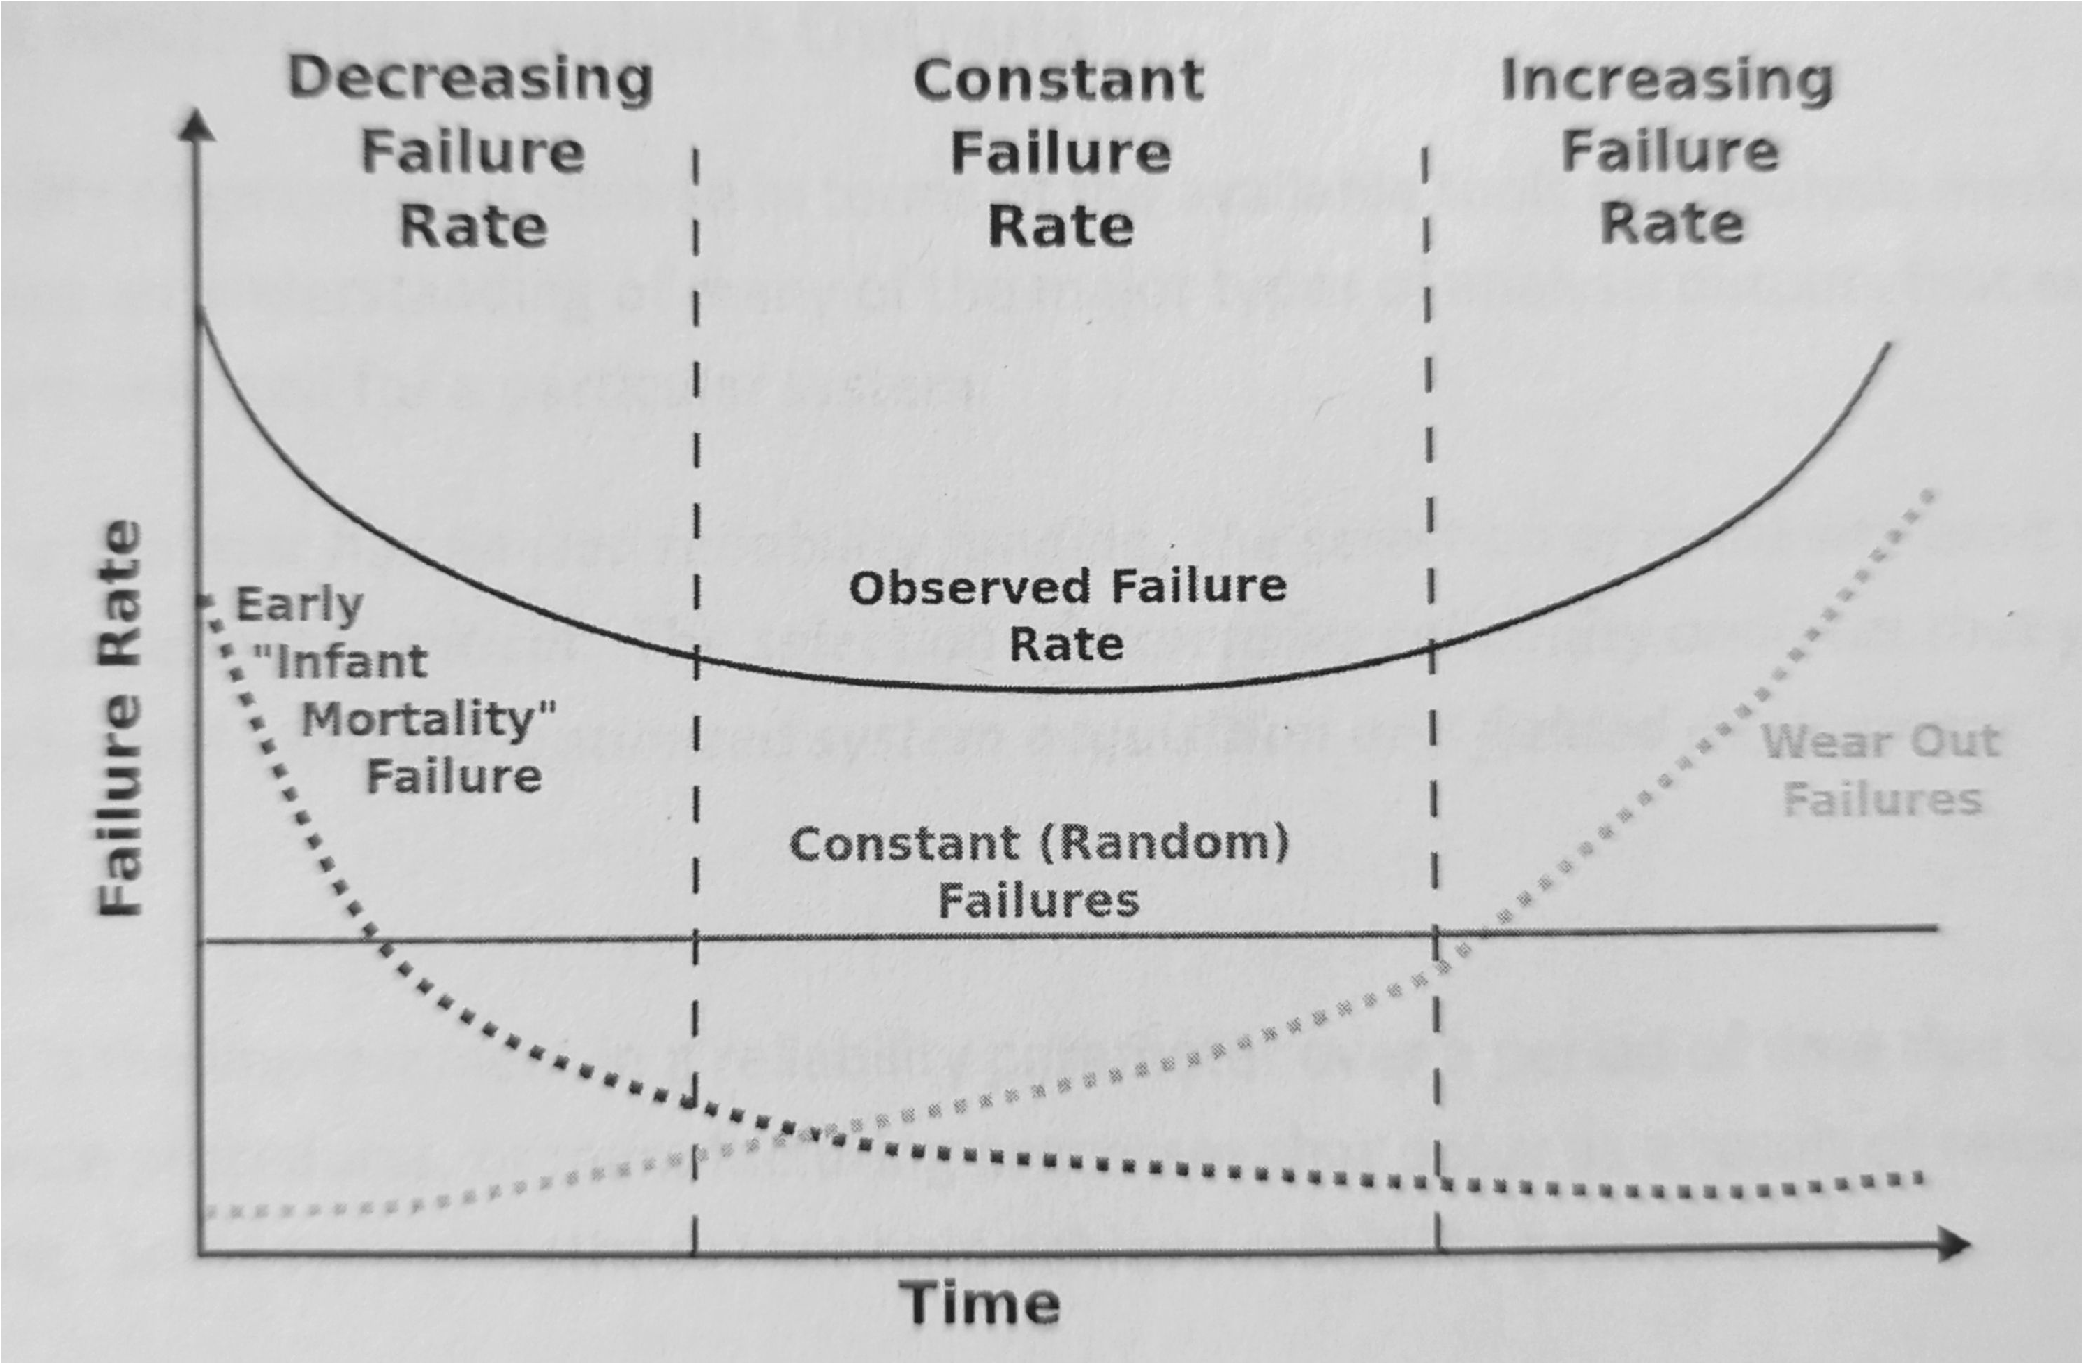
\includegraphics[width=0.55\linewidth]{bathtubCurve.pdf}
\end{figure}
\end{frame}

\begin{frame}{Module 1.1.2 : Impact of Reliability}
\small
\textbf{Reliability can grow by acting on analysis.}
\begin{itemize}
\scriptsize
\item \textbf{Reliability growth : } is an improvement in a reliability parameter over a period of time, driven by reliability growth programs (RGPs).
\begin{itemize}
\scriptsize
\item \textit{Failure Modes Effects Analysis (FMEA/FMECA)} (criticality)
\item \textit{Faiilure Report Analysis and Corrective Action System (FRACAS)}
\end{itemize}
\end{itemize}
\begin{figure}
\centering
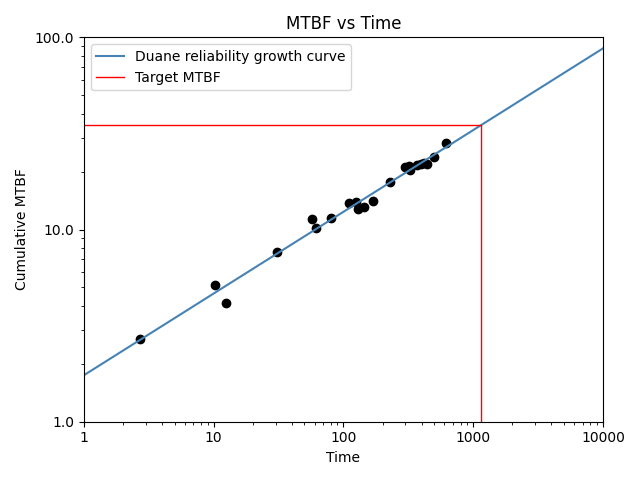
\includegraphics[width=0.6\linewidth]{r_growth.png}
\end{figure}
\end{frame}

\begin{frame}{Module 1.1.2 : Impact of Reliability}
\small
\textbf{Other common terminology in reliability :}
\begin{itemize}
\scriptsize
\item \textit{Maintenance policy optimization :} analysis of maintenance procedures, including sparing, personnel, and transportation, to meet reliability requirement
\item \textit{Reliability predictions :} calculations and simulations of reliability parameters that lead to system insights
\item \textit{System availability :} quantifies how well systems are maintained such that they are ready to deploy.  Depends on system type and is distinct from reliability measures.
\item \textit{Stockpile availability :} similar to system availability, but targets sub-groups of assests, rather than the entire set of assets.
\end{itemize}
\end{frame}

\begin{frame}{Module 1.1.3 : Knowing Our Systems}
\textbf{System Types}
\begin{itemize}
\small
\item \textbf{Continuous Use : } These systems are maintained so that reliability parameters can be determined with continuous functions.
\begin{itemize}
\small
\item Time to failure or time between repair data
\item Potential failure data can be right-censored if it is unknown when the asset will fail in the future.
\end{itemize}
\item \textbf{One-Shot/Impulse Untestable :} The reliability of these systems cannot be measured until the system is deployed irreversibly.
\begin{itemize}
\small
\item Failures are left-censored if it is unknown when the asset first failed.
\item Potential failure data can be right-censored if it is unknown when the asset will fail in the future.
\end{itemize}
\end{itemize}
\end{frame}

\begin{frame}{Module 1.1.3 : Knowing Our Systems}
\textbf{System Types}
\begin{itemize}
\small
\item \textbf{Impulse Testable : } These systems are maintained in such a way that they are known to be good at the last time they were tested.
\begin{itemize}
\small
\item Assets are often periodically certified.
\item The data is interval censored, from the right and the left.
\end{itemize}
\end{itemize}
\end{frame}

\begin{frame}{Module 1.1.3 : Knowing Our Systems}
\small
\textbf{Data is the foundation of reliability assessment}
\begin{itemize}
\scriptsize
\item Reliability analysis requires data describing the system state at known times.
\item Data from identical systems tested under similar conditions is preferred.
\item When necessary, data from similar systems or operating conditions can be used, if statistical techniques account for the differences.
\item SME (Subject Matter Expert) estimates should be used when data are unavailable.
\end{itemize}
\textbf{Common reliability data types:}
\begin{itemize}
\scriptsize
\item \textit{Priors:} Historical data or SME estimates used to constrain Bayesian models.
\item \textit{Historical:} Data from nearly identical or identical previous systems/components.
\item \textit{Time-to-Failure or Repair:} Operating time until failure or repair, including right-censored observations.
\end{itemize}
\end{frame}

\begin{frame}{Module 1.1.3 : Knowing Our Systems}
\begin{figure}
\centering
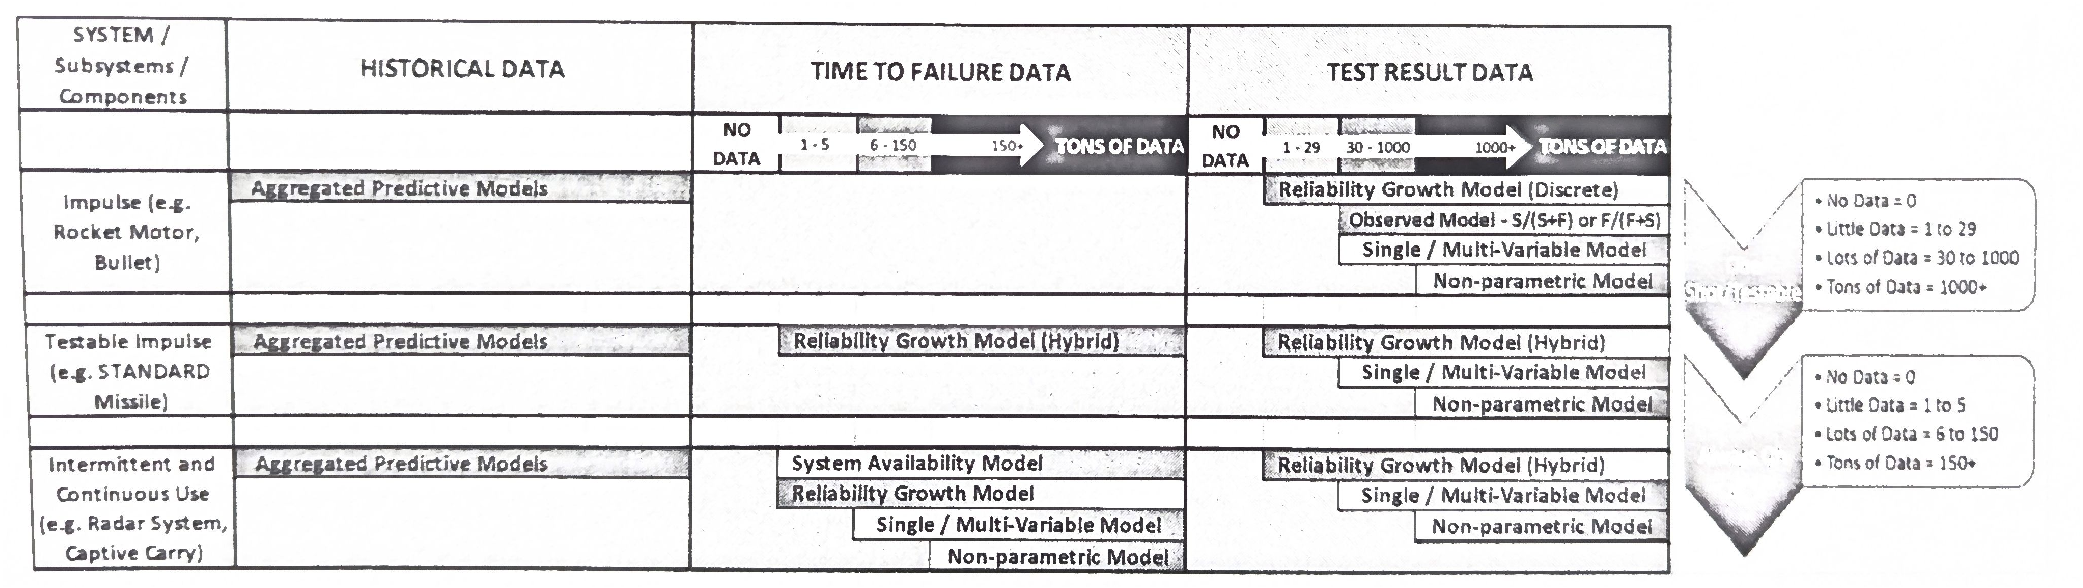
\includegraphics[width=0.99\linewidth,trim=0cm 0cm 6.8cm 0cm,clip=true]{r_data.pdf}
\caption{System type versus reliability data type, and notes.  Source: ``A Simplified Technical Guide for System Reliability: A Reliability Planning and Deployment Reference for Acquisition Professionals.'' (Section 219 Project, 2019, Port Hueneme/NAWC China Lake/NSWC Corona).}
\end{figure}
\end{frame}

\begin{frame}{Module 1.1.3 : Knowing Our Systems}
\small
\textbf{Successful reliability programs require skilled personnel, appropriate data, software tools, and computing resources.} \\ \vspace{0.25cm}
\scriptsize
\textbf{Reliability Modeling}
\begin{itemize}
\scriptsize
\item Skills/Personnel: knowledge of system components, statistics, systems engineering, modeling expertise, software proficiency
\item Resources: scored reliability data, modeling software, computing resources
\end{itemize}
\textbf{Data Scoring \& Evaluation}
\scriptsize
\begin{itemize}
\item Skills/Personnel: system familiarity, to classify valid failures vs.\ unusable data
\item Resources: production/in-service test data, environmental data, reliability databases, computing resources
\end{itemize}
\textbf{Reliability Analysis}
\begin{itemize}
\item Skills/Personnel: engineering, statistics, modeling, and logistics
\item Resources: validated reliability models, analysis software, computing resources
\end{itemize}
\end{frame}

\begin{frame}{Module 1.1.4 : Reliability Model and Method Selection}
\textbf{Five main questions to ask : }
\begin{enumerate}
    \item What are your program reliability requirements?
    \item What is your system type?
    \item What types of system data do you have?
    \item How much data do you have?
    \item In what phase of the life-cycle is your system?
\end{enumerate}
\end{frame}

\begin{frame}{Module 1.1.4 : Reliability Model and Method Selection}
\scriptsize
\textbf{Predictive Reliability Models: Aggregated (``Roll-Up'') Models}
\begin{itemize}
\scriptsize
\item Combine subsystem reliability estimates to predict overall system reliability.
\item Common methods: MIL-HDBK-217 predictions, Reliability Block Diagrams (RBD)
\end{itemize}
\textbf{Example Reliability Roll-Up}
\begin{center}
\begin{tabular}{|l|c|c|}
\hline
\textbf{Subsystem} & \textbf{Reliability} & \textbf{Running R} \\
\hline
Power Supply & 0.995 & 0.995\\
Processor    & 0.990 & 0.985 \\
Communications & 0.985 & 0.970 \\
Sensors      & 0.980 & 0.951 \\ \hline
\textbf{System} & $R_{\rm sys}=\prod_i R_i$ & \textbf{0.951} \\
\hline
\end{tabular}
\end{center}
\vspace{0.25cm}
\begin{columns}[T]
\begin{column}{0.48\textwidth}
\textbf{Benefits}
\begin{itemize}
\item Simple calculations and minimal data requirements
\item Can leverage historical data
\item Supports reliability allocation during design
\end{itemize}
\end{column}
\begin{column}{0.48\textwidth}
\textbf{Limitations}
\begin{itemize}
    \item Accuracy depends on subsystem models
    \item Error propagation leads to inaccuracies or imprecision for system performance
\end{itemize}
\end{column}
\end{columns}
\end{frame}

\begin{frame}{Module 1.1.4 : Reliability Model and Method Selection}
\scriptsize
\textbf{Reliability Growth Models}
\begin{itemize}
\scriptsize
\item Model improvements in system reliability as failures are identified and corrected during testing.
\item Common methods: Crow-AMSAA, Duane Model, and accelerated life testing (HALT/HASS).  The example below reflects Crow-AMSAA method, with $\text{Cumulative MTBF} = \text{Cumulative Hours}/\text{Cumulative Failures}$.
\end{itemize}
\begin{center}
\begin{tabular}{|c|c|c|c|}
\hline
\textbf{Test Hours} & \textbf{Cumulative Failures} & \textbf{Cumulative MTBF (hr)} & \textbf{Running Growth} \\
\hline
100  & 10 & 10.0 & 1.00 \\
300  & 20 & 15.0 & 1.50 \\
700  & 35 & 20.0 & 2.00 \\
1500 & 50 & 30.0 & 3.00 \\
\hline
\end{tabular}
\end{center}
\vspace{0.25cm}
\begin{columns}[T]
\begin{column}{0.48\textwidth}
\textbf{Benefits}
\begin{itemize}
\item Quantifies reliability improvement
\item Measures effectiveness of corrective actions during testing
\item Supports reliability planning
\end{itemize}
\end{column}
\begin{column}{0.48\textwidth}
\textbf{Limitations}
\begin{itemize}
\item Requires representative data
\item Assumes corrective actions are implemented
\item Predictions depend on test conditions and reporting
\end{itemize}
\end{column}
\end{columns}
\end{frame}

\begin{frame}{Module 1.1.4 : Reliability Model and Method Selection}
\scriptsize
\textbf{Reliability Growth Models}
\begin{itemize}
\scriptsize
\item Model improvements in system reliability from corrective actions during testing.
\item Common methods: Crow-AMSAA (continuous and discrete), Duane Model, and accelerated life testing (HALT/HASS/TAAF).
\end{itemize}
\begin{figure}
\centering
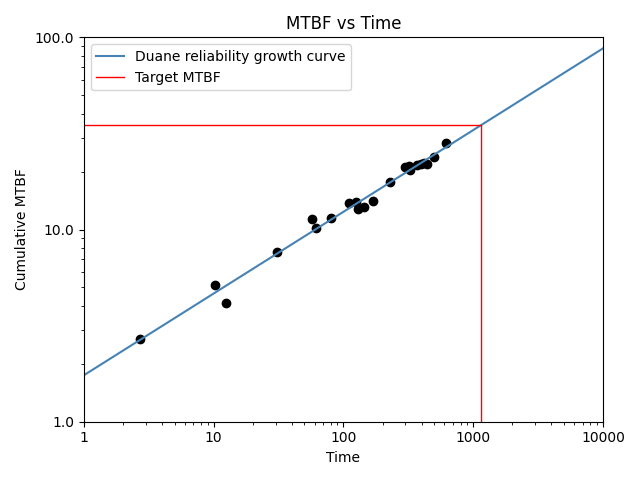
\includegraphics[width=0.6\linewidth]{r_growth.png}
\end{figure}
\end{frame}

\begin{frame}{Module 1.1.4 : Reliability Model and Method Selection}
\scriptsize
\textbf{System Availability Model}
\begin{itemize}
\scriptsize
\item Model probability that systems are available for operation at an arbitrary time.
\item Examples: $A_O = \text{Uptime}/(\text{Uptime}+\text{Downtime})$, Markov Modeling
\end{itemize}
\vspace{0.25cm}
\begin{columns}[T]
\begin{column}{0.48\textwidth}
\textbf{Benefits}
\begin{itemize}
\item Well-defined with low data requirements
\item Works for most continuous and impulse testable systems 
\end{itemize}
\end{column}
\begin{column}{0.48\textwidth}
\textbf{Limitations}
\begin{itemize}
\item Not well-defined for impulse untestable systems
\end{itemize}
\end{column}
\end{columns}
\rule{\textwidth}{0.5pt}
\textbf{Single/Multivariable Model}
\begin{itemize}
\scriptsize
\item Mathematical equations that model reliability versus time and other factors
\item Examples: Exponential and Weibull models
\end{itemize}
\vspace{0.25cm}
\begin{columns}[T]
\begin{column}{0.48\textwidth}
\textbf{Benefits}
\begin{itemize}
\item Accurate, precise, supports numerical analysis
\item Identification of key parameters
\end{itemize}
\end{column}
\begin{column}{0.48\textwidth}
\textbf{Limitations}
\begin{itemize}
\item Requires larger data sets, knowledge of statistical and computational techniques
\end{itemize}
\end{column}
\end{columns}
\end{frame}

\begin{frame}{Module 1.1.5 : Model Development}
\small
\textbf{Data is the fundamental driving force for reliability analysis.}
\begin{itemize}
\small
\item Data is often not cheap
\item Carefully consider data acquisition
\begin{itemize}
\small
\item Depends on system type (impulse untestable, impulse testable, continuous)
\end{itemize}
\end{itemize}
\textbf{Examples of data items:}
\begin{itemize}
\small
\item Pass or Fail data (T and E data)
\item Failure Reporting and Corrective Action System (FRACAS)
\item Hardware specifications, configuration data, inventory tracking
\item Material transfer and transport information
\end{itemize}
\textbf{Develop the data that is necessary to achieve reliability goals}
\end{frame}

\begin{frame}{Module 1.1.5 : Model Development}
\small
\textbf{Data drives model development.}
\begin{itemize}
\small
\item Some reliability models require time-dependent data
\item Some reliability models require pass-fail data
\item Data type can evolve over time - reliability models evolve with it
\end{itemize}
\textbf{Hardware drives model development.}
\begin{itemize}
\small
\item Engineering community and subject matter experts (SMEs) can provide historical insight on known components
\item System designs map to tools like RBDs, and fault/success trees
\end{itemize}
\textbf{Models that provide quantitative point estimates and confidence limits for reliability parameters are preferred}
\end{frame}

\begin{frame}{Module 1.1.5 : Model Development}
\small
\textbf{Reliability models should be validated.}
\begin{itemize}
\small
\item Examples of comparison between model and reality
\begin{itemize}
\small
\item Graph data on the same axes as model prediction
\item Calculate goodness of fit between data and model
\end{itemize}
\item Peer review
\begin{itemize}
\small
\item Portions of the model may be generalized and unclassified
\item These can be compared to other published research
\item New techniques can be published and scrutinized
\end{itemize}
\end{itemize}
\end{frame}

\begin{frame}{Module 1.1.5 : Model Development}
\textbf{Example matrix for Reliability Model Selection}
\begin{figure}
\centering
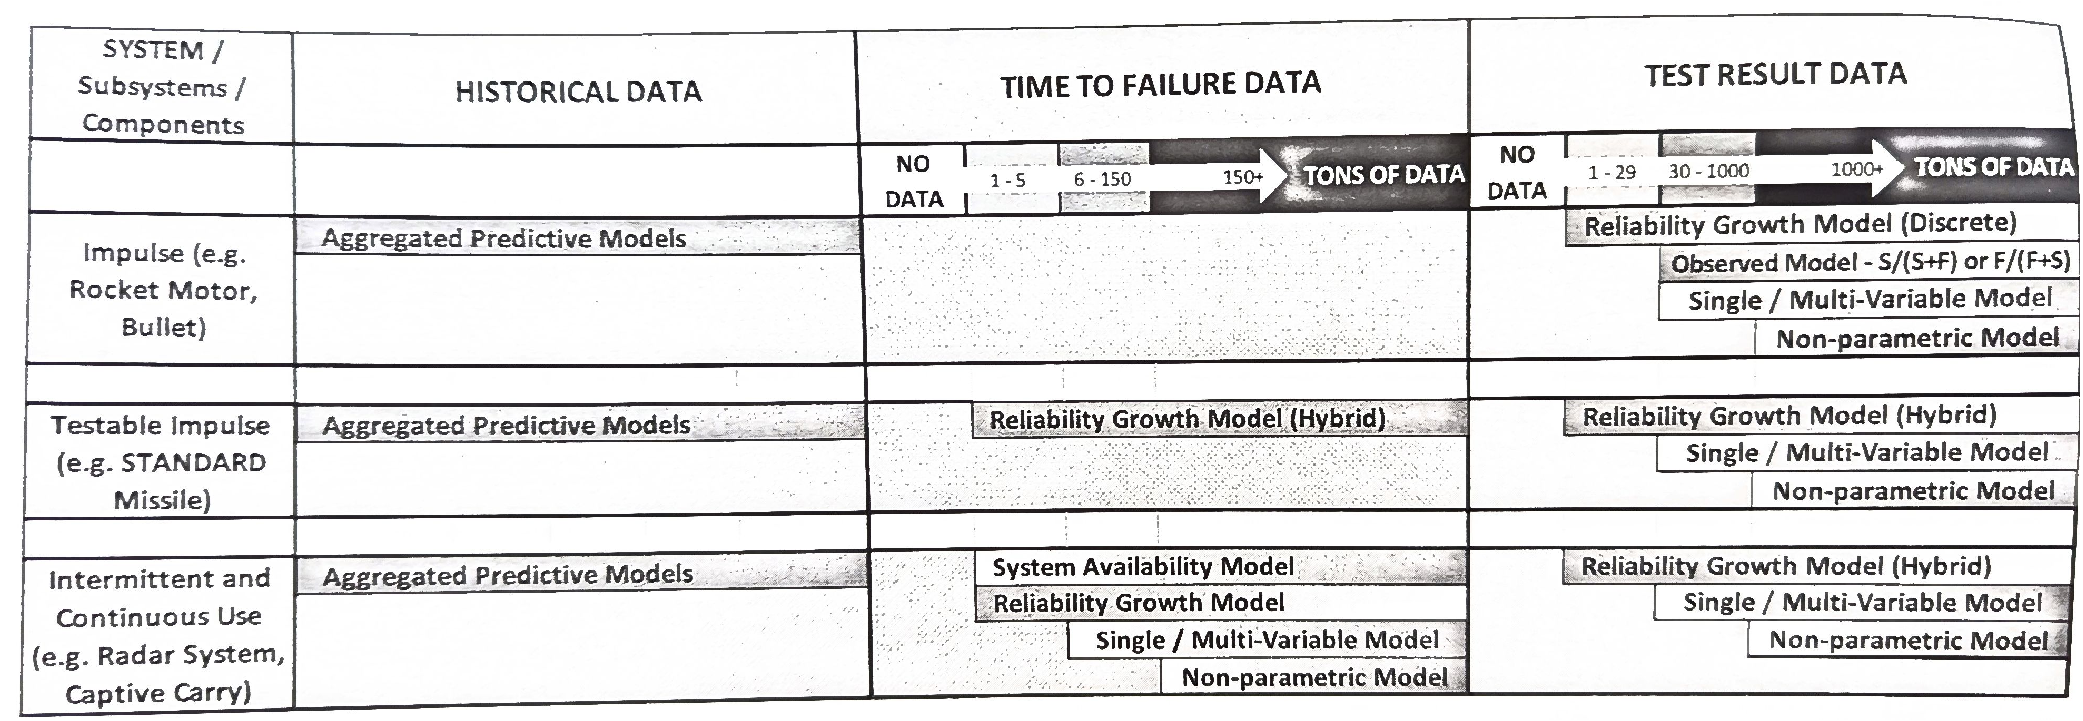
\includegraphics[width=0.95\linewidth]{r_select.pdf}
\end{figure}
\end{frame}

\end{document}